\documentclass{physlab}
%%%%
\usepackage[utf8]{inputenc}
\usepackage[russian]{babel}
\usepackage{amsmath}
\usepackage{amsfonts}
\usepackage{amssymb}
\usepackage{amsthm}
\usepackage{mathtools}
\usepackage{misccorr}
\usepackage{indentfirst}
\usepackage{multirow}
\usepackage{wrapfig}
\usepackage{graphicx}
%\usepackage{subfig}
\usepackage{adjustbox}
\usepackage{pgfplots}
\usepackage{geometry}
\usepackage{comment}
\usepackage{hyperref}


\graphicspath{{graphs/}}
\geometry{top=20mm}
\geometry{bottom=20mm}
\geometry{left=20mm}
\geometry{right=20mm}

% объявляем новую команду для переноса строки внутри ячейки таблицы
\newcommand{\specialcell}[2][l]{%
	\begin{tabular}[#1]{@{}l@{}}#2\end{tabular}}
\DeclareMathOperator*{\argmin}{arg\,min}

\begin{document}
	
	\title{	Алгоритмы сокращения пространства поиска на графе регулярной декомпозиции за счет симметрии и смежных техник (JPS и его модификации). \\
	
	\href{https://github.com/Ilyabasharov/path_planning}{GitHub}.
	
}
	\author{Трясогузов Павел, Башаров Илья}
	\date{\today}
	
	\maketitle

\tableofcontents % это оглавление, которое генерируется автоматически


\section{Введение}
Существует много алгоритмов для поиска кратчайшего пути на 2D сетке. Алгоритм A* является самым простым и известным из них. В настоящее время известно достаточно много модификаций этого алгоритма. Одной из лучших модификаций на сегодняшний день является Jump Point Search. Данный алгоритм является улучшенным алгоритмом поиска пути A*. JPS ускоряет поиск пути, “перепрыгивая” многие места, которые должны быть просмотрены.  В отличие от подобных алгоритмов JPS не требует предварительной обработки и дополнительных затрат памяти. Данный алгоритм представлен в 2011 году, а в 2012 получил высокие отклики. \\


\section{Терминалогия}
Алгоритм работает на неориентированном графе единой стоимости. Каждое поле карты может иметь не более 8 соседей, которые могут быть проходимы или нет. Каждый шаг по направлению (по вертикали или по горизонтали) имеет стоимость 1; шаг по диагонали имеет стоимость $\sqrt{2}$. Движения через препятствия запрещены. Обозначение  относится к одному из восьми направлений движения (вверх, вниз, влево и т.д.). 
\begin{itemize}
    \item $p = (n_{0}, n_{1},...,n_{k})$ - упорядоченное перемещение по точкам без циклов из вершины $n_{0}$ до вершины $n_{k}$
    \item $p\backslash x$ - отсутствие вершины x в пути p
    \item $len(p)$ - стоимость (длина) пути p
    \item $dist(x, y)$ - длина (стоимость) пути между вершинами x и y

\end{itemize}
\textbf{Определение 1.} \\
Вершина $n \in neighbours(s)$ является принужденной, если 
\begin{enumerate}
    \item n - неестественный сосед x
    \item $len((p(x),..,n) \backslash x) < len(p(x), x, n)$
\end{enumerate}

\begin{figure}[H]
\begin{minipage}[h]{0.55\linewidth}
\center{\includegraphics[width=0.4\linewidth]{1а.png} \\}
\subcaption{Прямолинейнное перемещение (принужденный сосед -3)}
\end{minipage}
\hfill
\begin{minipage}[h]{0.44\linewidth}
\center{\includegraphics[width=0.43\linewidth]{1б.png} \\}
\subcaption{Диагональное перемещение (принужденный сосед -1)}
\end{minipage}
\caption{Примеры принужденных соседей}
\end{figure} 

\textbf{Определение 2.} \\
Вершина y называется точкой прыжка вершины x, в направлении d, если  $y = x + kd$, и выполняется одно из следующих условий:
\begin{enumerate}
    \item y - целевая вершина
    \item вершина y имеет хотя бы одного соседа, который является принужденным по определению 1.
    \item d - движение по диагонали и существует вершина $z = y + k_{i} d_{i}$, которая лежит в $k_{i}$ шагах в направлении $d_{i} \in \{d_{1}, d_{2} \}$, таких что z - точка прыжка из y при условии 1 или 2.
\end{enumerate}

\begin{figure}[H] 
\centering
    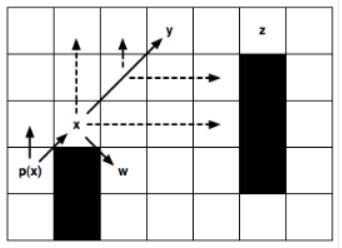
\includegraphics[width=0.4\linewidth]{2.png}
    \caption{Примеры точек прыжка.}
\end{figure}

\section{Постановка задачи}
Целью данной работы является исследование алгоритма Jump Point Search, а также его различные модификации (JPS+, JPS+BB). 

\section{Описание алгоритма Jump Point Search}
Основная идея алгоритма Jump Point Search заключается в том, что если мы будем добавлять в открытый список только точки "прыжка"\ вершины, а не всех соседей данной вершины, то значительно ускорим алгоритм поиска основанный на $A^{*}$. Такие точки описываются двумя простыми правилами выбора соседей при рекурсивном поиске: одно правило для прямолинейного движения и другое – для диагонального. В обоих случаях можно показать, что для отсеченных (невыбранных) соседей вокруг рассматриваемой вершины, найдётся оптимальный путь из предка текущей вершины до каждого из соседей, и этот путь не будет содержать в себе посещенную точку. 
\begin{figure}[H]
\begin{minipage}[h]{0.55\linewidth}
\center{\includegraphics[width=0.4\linewidth]{5а.png} \\}
\subcaption{Прямой переход}
\end{minipage}
\hfill
\begin{minipage}[h]{0.55\linewidth}
\center{\includegraphics[width=0.4\linewidth]{5б.png} \\}
\subcaption{Диагональный переход}
\end{minipage}
\caption{Правила отсечки}
\end{figure} 
Таким образом наша цель заключается в ликвидации "симметрии"\ , рекурсивно "перепрыгивая"\ через все вершины, в которые можно попасть по оптимальному пути, который не проходил через текущую позицию. Рекурсия останавливается при попадании на препятствие или если мы нашли так называемую "прыжковую точку-преемник" (jump point successor). Прыжковые точки интересны тем, что они имеют соседей, которые не могут быть достигнуты альтернативным путём: оптимальный путь должен идти через текущую точку Рис. 3. 

\textbf{Входные данные}: точка старта, точка финиша\\
\textbf{Выходные данные}: кратчайший путь из точки старта в точку финиша
\begin{figure}[H]
\begin{minipage}[h]{0.55\linewidth}
\center{\includegraphics[width=1.\linewidth]{4а.png} \\}
\subcaption{Функция определения successors}
\end{minipage}
\hfill
\begin{minipage}[h]{0.44\linewidth}
\center{\includegraphics[width=1.\linewidth]{4б.png} \\}
\subcaption{Функция "прыжка"}
\end{minipage}
\caption{Алгоритм Jump Point Search}
\end{figure} 
Псевдокод алгоритма Jump Point Search представлен на Рис. 4.  Функция определения приемников (successors)  показывает как искать преемника для текущей вершины. Сначала обрезается множество соседей, непосредственно примыкающих к текущей вершине х. Затем используем функцию "прыжка"  для поиска вершины, которая находится дальше ближайщего соседа x - n, но которая лежит относительно направления x к n. Если находится такая точка, то она добавляется в набор преемников (successors) вместо n. Если до точки прыжка дойти не получается, то ничего не добавляется. Процесс продолжается до тех пор, пока все соседи не закончатся, и затем алгоритм вернёт список всех преемников для х. \\
Для того, чтобы найти отдельных преемников для точки прыжка, испоьзуется функция "прыжка" (function jump). Входные параметры данной функции - текущая вершина x, направление движения d, а так же начальная вершину s и целевая вершину g. Алгоритм пытается установить, имеет ли x точку для прыжка среди своих преемников, перемещается по направлению d  и проверяет, удовлетворяет ли точка n \textbf{Определению 2}. Если n явялется точкой "прыжка", то она возращается, иначе алгоритм рекурсивно повторяется и двигается снова в направлении d, но в этот раз n – новая точка отсчёта. Рекурсия прекращается, когда встречается препятствие и никакие дальнейшие действия не могут быть предприняты. Стоит обратить внимание, что перед каждым диагональным шагом алгоритм должен обнаружить точки прыжка по прямым направлениям. Эта проверка соответствует третьему условию \textbf{Определения 2} и имеет важное значение для сохранения оптимальности алгоритма.

\section{Описание алгоритма Jump Point Search +}
\begin{figure}[H]
\begin{minipage}[h]{0.50\linewidth}
\center{\includegraphics[width=0.96\linewidth]{6а.jpg} \\}
\subcaption{Точки прыжка, вычисленные для данной карты, для вершины N предварительно}
\end{minipage}
\hfill
\begin{minipage}[h]{0.48\linewidth}
\center{\includegraphics[width=0.97\linewidth]{6б.jpg} \\}
\subcaption{Процесс генерации целевой точки прыжка}
\end{minipage}
\caption{}
\end{figure} 
Одной из важных модификацией алгоритма JPS является алгоритм JPS+. Ключевая особенность данного метода состоит из предобработки исходной карты. Принцип преобработки заключается в том, что для каждой вершины мы отмечаем расстояния до всех ближайших точек прыжка по всем направлениям, на рис 5.а для вершины N точки 1-3 являются прыжковыми, кроме того, если нет прыжковой точки по заданному направлению, то добавляется вершина, граничащая с блоком или концом карты по заданному направлению. Таким образом формируется множество всех возможных приемников для каждой из вершины. Также стоит отметить, что для того, чтобы избежать перепрыгивания целевой точки (рис. 5б) при выборе приемников неоходимо генерировать целевые точки прыжка, на рис 5.б показано создание такой точки, вершина S - приемник N, при переходе из N в S создается вершина J, которая находится на пересечении перехода N-S одной из координат целевой точки.

\section{Прунинг: Bounding Boxes}
Прунинг или отсечение - техника фильтрации предполагаемых преемников на этапе их генерации. Главная цель техники - создать ограничивающее поле для каждого из наследников таким образом, чтобы в нем находились только те точки, до которых можно добраться оптимальным образом из любой точки внутри прямоугольника. Проделав данную предобработку, мы сможем оценивать, сможет ли текущий преемник достигнуть финиша или нет за O(1).

Главная проблема подхода - долгое время предподсчета. Необходиомо найти оптимальный путь от каждой вершины до каждой. Главным методом предподсчета будет являться алгоритм Дейкстры. Таким образом, общее время предподсчета составит $O(n^2logn)$, где $n$ - число узлов сетки.

\section{Результаты экспериментальных исследований}
Эксперименты проводились на двух картах Dragon Age из moving AI. Были выбраны легкие и сложные карты для тестирования для того, чтобы показать различия в работе алгоритмов. Основное отличие карт в количесве препятствий. Анализ времени выолнения для карты №1 представлен на рис. 6. На рис. 6а можно заметить, что для JPS дает улучшение времени работы в 1.8 раз по сравнению с алгоритмом Astar, в то время как алгоритм JPS+ сокращает время выполения значительно (в 10 раз по сравнению с JPS). На рис. 6б приведен приведен график для алгоритмов  с использованием прунинга, техника BBox уменьшает время работы алгоритмов Astar и JPS в 10 раз, в случае с JPS+ - в 1.5 раза.  
\begin{figure}[H]
	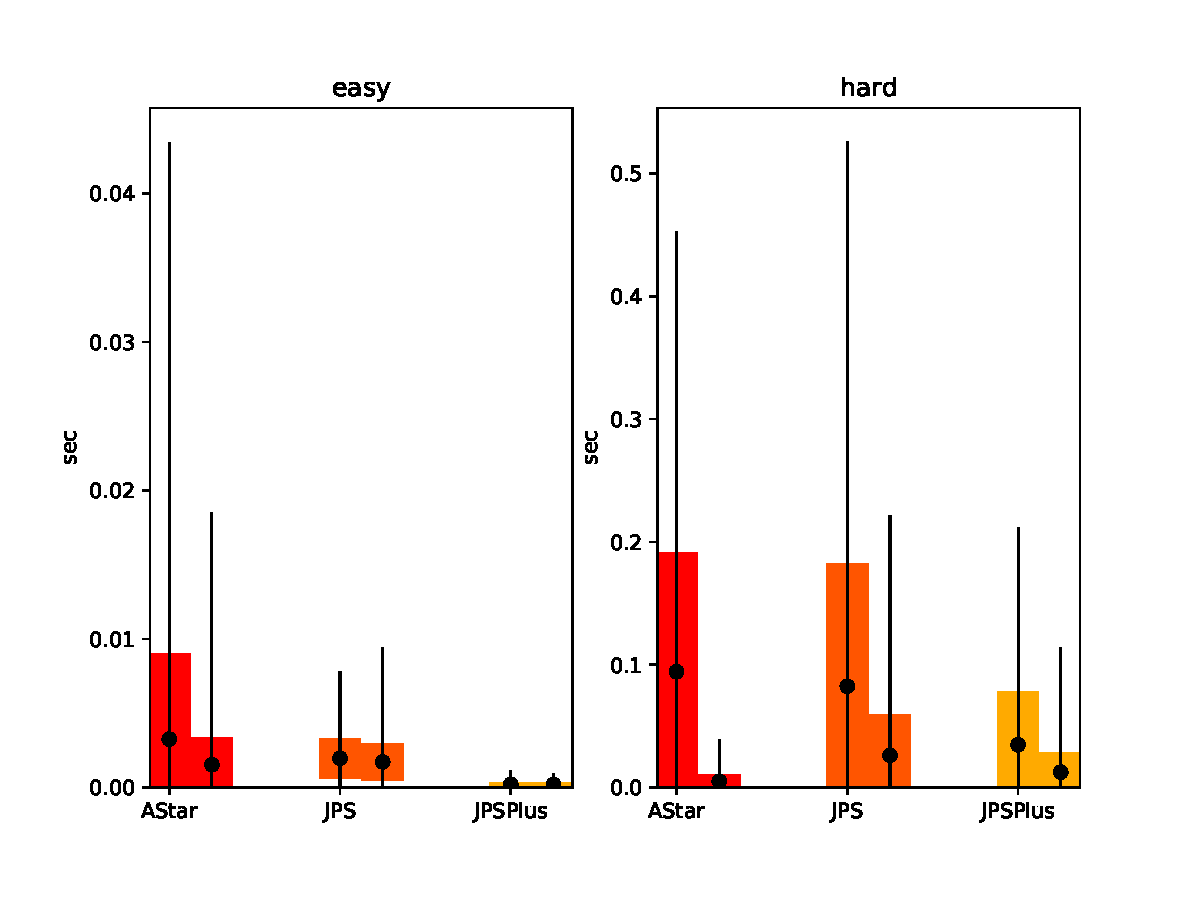
\includegraphics[width=0.93\linewidth]{error.pdf}
\caption{Время выполения для карты № 1.}
\end{figure} 
На рис. 7 представлены графики зависимости длины пути от времени. Как можно заметить алгоритм JPS+ наименее чувствителен к росту длины пути на данных картах. 
\begin{figure}[H]
	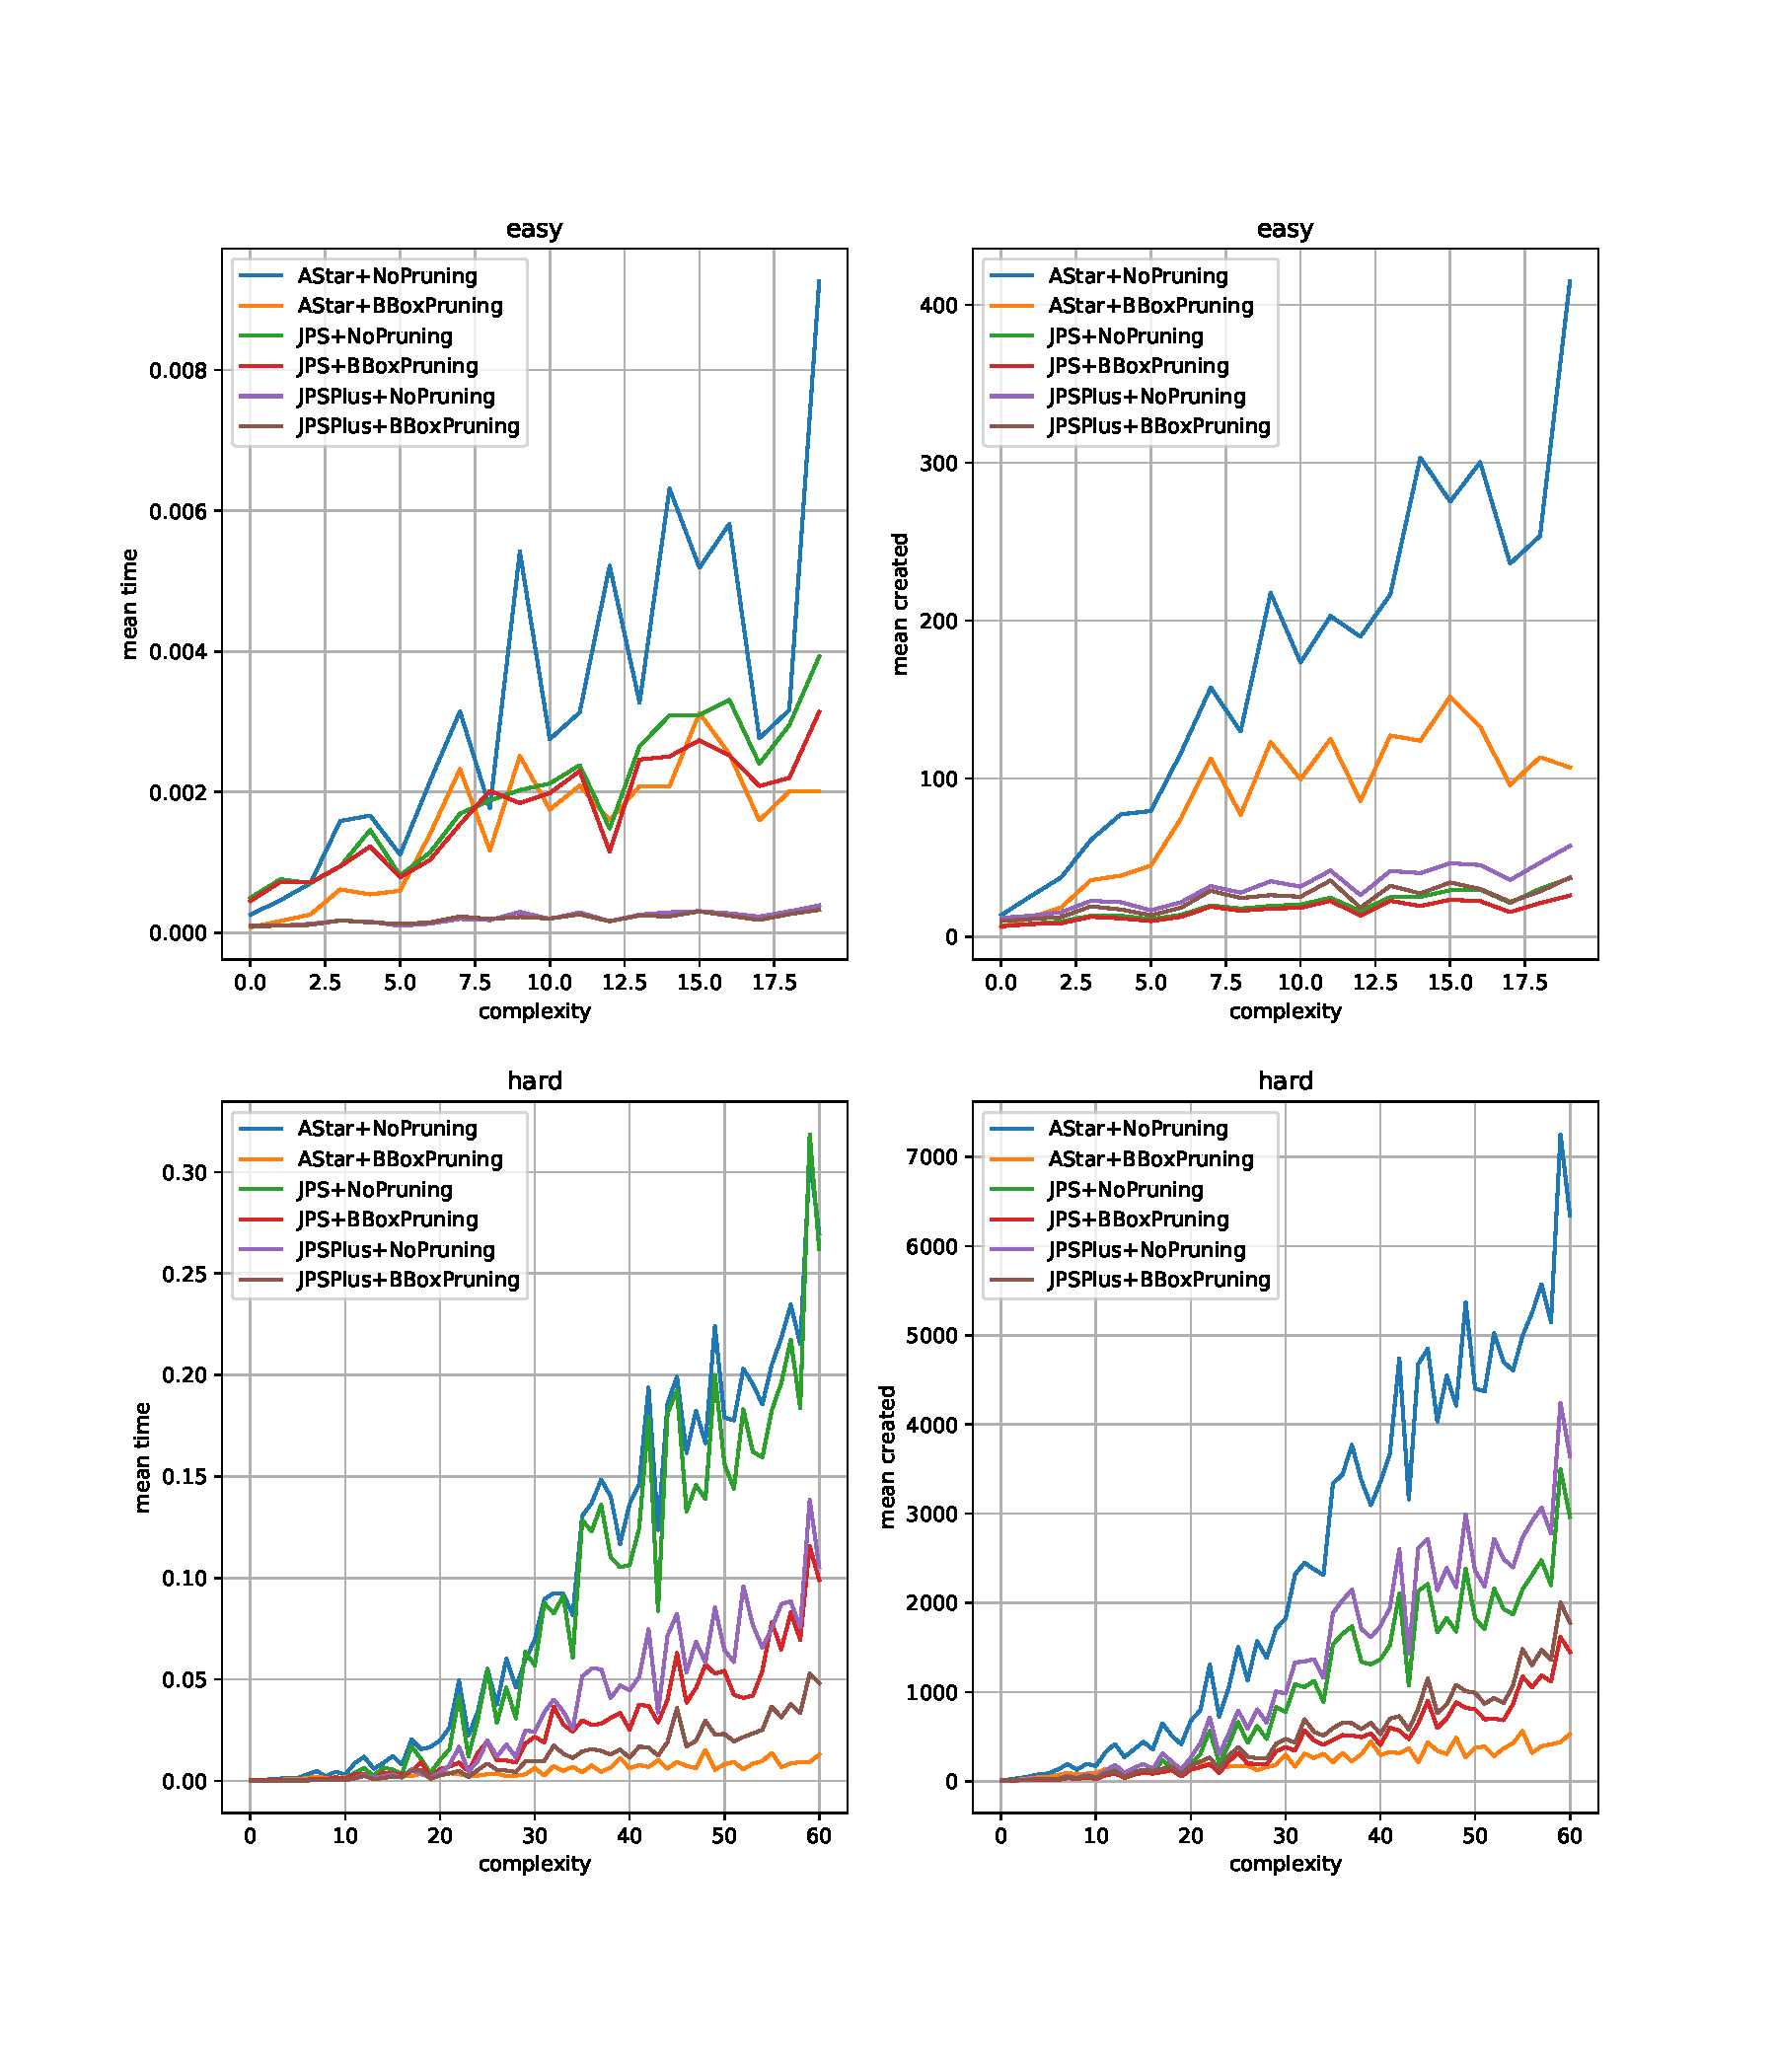
\includegraphics[width=0.93\linewidth]{comparison.pdf}
\caption{Зависимость среднего времени и количества нодов от сложности задания}
\end{figure} 



\section{Литература}
\begin{itemize}
    \item Harabor, D. and Grastien, A., 2011: Online graph pruning for pathfinding on grid maps (JPS)
    \item Harabor, D. and Grastien, A., 2014: Improving jump point search (JPS+)
    \item Rabin, S. and Sturtevant, N., 2016: Combining bounding boxes and JPS to prune grid pathfinding (JPS+BB)
    \item Sturtevant, N.R. and Rabin, S., 2016: Canonical orderings on grids
\end{itemize}
    
\end{document}